\section{Proposed architecture}
Our mushroom classification model utilizes the EfficientNetB0 architecture, renowned for its efficiency and performance in image classification tasks. Fine-tuning the pre-trained EfficientNetB0 model on our dataset allows it to adapt its parameters to the specific task of mushroom classification while leveraging knowledge learned from large-scale image datasets.
EfficientNet architecture consists of seven blocks which are shown in different colours. The basic building block of EfficientNet-B0 is a mobile inverted bottleneck convolution (MBConv), while each MBConv block is shown with the corresponding kernel filter size \cite{zhou2022multihead}. The figure below shows the different block:

\begin{figure}[!ht]
    \centering
    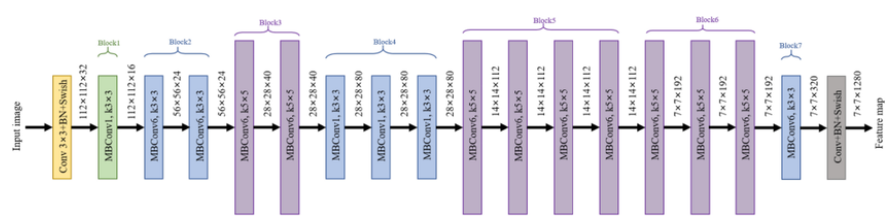
\includegraphics[height=6cm, width=9cm]{images/EfficientNet.PNG}
    \caption{Figure 3 from Zhou et al. (2022) illustrates the architecture of EfficientNetBO}
\end{figure}

The model comprises convolutional layers followed by depthwise separable convolutions. We modify this EfficientNetB0 by adding few layers and a classification layer. Global average pooling was used to reduce the parameter size. This layer not just reduce parameter also preserve the most important features by taking out the average. On top of that dense layer with ReLU activation was used further enhancing the model's ability to learn complex pattern in images, dropout regularization was used ensuring that the model could be generalized and does better on test set rather than just doing good only on training set. And a classification layer with sigmoid activation was used for binary classification. This architecture enables the development of a robust classification model capable of accurately distinguishing between edible and poisonous mushrooms.